\documentclass[a4paper,11pt]{article}
\usepackage{amsmath,amsthm,amsfonts,amssymb,amscd,amstext,vmargin,graphics,graphicx,tabularx,multicol} 
\usepackage[francais]{babel}
\usepackage[utf8]{inputenc}  
\usepackage[T1]{fontenc} 
\usepackage{pstricks-add,tikz,tkz-tab,variations}
\usepackage[autolanguage,np]{numprint} 

\setmarginsrb{1.5cm}{0.5cm}{1cm}{0.5cm}{0cm}{0cm}{0cm}{0cm} %Gauche, haut, droite, haut
\newcounter{numexo}
\newcommand{\exo}[1]{\stepcounter{numexo}\noindent{\bf Exercice~\thenumexo} : \marginpar{\hfill /#1}}
\reversemarginpar


\newcounter{enumtabi}
\newcounter{enumtaba}
\newcommand{\q}{\stepcounter{enumtabi} \theenumtabi)  }
\newcommand{\qa}{\stepcounter{enumtaba} (\alph{enumtaba}) }
\newcommand{\initq}{\setcounter{enumtabi}{0}}
\newcommand{\initqa}{\setcounter{enumtaba}{0}}

\newcommand{\be}{\begin{enumerate}}
\newcommand{\ee}{\end{enumerate}}
\newcommand{\bi}{\begin{itemize}}
\newcommand{\ei}{\end{itemize}}
\newcommand{\bp}{\begin{pspicture*}}
\newcommand{\ep}{\end{pspicture*}}
\newcommand{\bt}{\begin{tabular}}
\newcommand{\et}{\end{tabular}}
\renewcommand{\tabularxcolumn}[1]{>{\centering}m{#1}} %(colonne m{} centrée, au lieu de p par défault) 
\newcommand{\tnl}{\tabularnewline}

\newcommand{\bmul}[1]{\begin{multicols}{#1}}
\newcommand{\emul}{\end{multicols}}

\newcommand{\trait}{\noindent \rule{\linewidth}{0.2mm}}
\newcommand{\hs}[1]{\hspace{#1}}
\newcommand{\vs}[1]{\vspace{#1}}

\newcommand{\N}{\mathbb{N}}
\newcommand{\Z}{\mathbb{Z}}
\newcommand{\R}{\mathbb{R}}
\newcommand{\C}{\mathbb{C}}
\newcommand{\Dcal}{\mathcal{D}}
\newcommand{\Ccal}{\mathcal{C}}
\newcommand{\mc}{\mathcal}

\newcommand{\vect}[1]{\overrightarrow{#1}}
\newcommand{\ds}{\displaystyle}
\newcommand{\eq}{\quad \Leftrightarrow \quad}
\newcommand{\vecti}{\vec{\imath}}
\newcommand{\vectj}{\vec{\jmath}}
\newcommand{\Oij}{(O;\vec{\imath}, \vec{\jmath})}
\newcommand{\OIJ}{(O;I,J)}


\newcommand{\reponse}[1][1]{%
\multido{}{#1}{\makebox[\linewidth]{\rule[0pt]{0pt}{20pt}\dotfill}
}}

\newcommand{\titre}[5] 
% #1: titre #2: haut gauche #3: bas gauche #4: haut droite #5: bas droite
{
\noindent #2 \hfill #4 \\
#3 \hfill #5

\vspace{-1.6cm}

\begin{center}\rule{6cm}{0.5mm}\end{center}
\vspace{0.2cm}
\begin{center}{\large{\textbf{#1}}}\end{center}
\begin{center}\rule{6cm}{0.5mm}\end{center}
}



\begin{document}
\pagestyle{empty}
\titre{Contrôle 1  }{Nom :}{Prénom :}{Classe}{Date}


\vspace*{0.25cm}
\begin{flushleft}
\begin{tabular}{|m{9.5cm}|m{1.25cm}|m{1.25cm}|m{1.25cm}|m{1.25cm}|m{1.25cm}|}
\hline 
\textbf{Compétences} & \begin{center}
\textbf{N.E.}
\end{center} & \begin{center}
\textbf{M.I.}
\end{center} & \begin{center}
\textbf{M.F.}
\end{center}  & \begin{center}
\textbf{M.S.}
\end{center} & \begin{center}
\textbf{T.B.M.}
\end{center} \\ 
\hline 
Je dois savoir produire et utiliser diverses représentations des fractions simples et des nombres décimaux &  &  & & &\\
\hline 
Je dois savoir placer un nombre sur demi-droite graduée &  &  & & &\\
\hline 
Je dois savoir additionner ou soustraire des nombres entiers et des nombres décimaux (calcul mental, posé ou en ligne) &  &  & & &\\
\hline


\end{tabular} 
\end{flushleft}

\textit{N.E = Non évalué ; M.I. = Maîtrise insuffisante ; M.F. = Maîtrise fragile ; M.S. = Maîtrise satisfaisante ; T.B.M. = Très bonne maîtrise}\\




\vspace*{0.15cm}


\textbf{Les exercices avec le symbole 
\includegraphics[scale=0.4]{trefle.eps} sont à faire directement sur le sujet. Les autres sont à faire sur la copie double.}\\





\vspace*{0.35cm}






\exo{4}
\includegraphics[scale=0.4]{trefle.eps} La première ligne de ce tableau est déjà complétée, à vous de finir de compléter le tableau. Chaque ligne correspond à un nombre différent.\\

\renewcommand{\arraystretch}{3}

\begin{flushleft}
\begin{tabular}{|p{2cm}|p{5cm}|p{5.5cm}|p{3.5cm}|}
\hline 
\textbf{Écriture décimale} & \textbf{Écriture en toutes lettres} & \textbf{Somme d'un nombre entier et d'une fraction décimale} & \textbf{Une seule fraction décimale} \\ 
\hline 
\begin{center}
 9,103
 \end{center} & Neuf unités et cent trois millièmes & \begin{center}
 $9 + \dfrac{103}{1000}$
 \end{center} &\begin{center}
  $\dfrac{9 103}{1000}$
 \end{center}  \\
 \hline 
\begin{center}
 3,7
 \end{center} & Trois unités et sept dixièmes &  &  \\ 
\hline 
 & Cinquante unités et quinze centièmes &  &  \\ 
\hline 
 &  &\begin{center}
  $5 + \dfrac{82}{1000}$
 \end{center} &  \\ 
\hline 
\end{tabular} 
\end{flushleft}



\newpage


\exo{3} Gaëlle a été absente au cours de mathématiques vendredi dernier. Écrire le programme de construction qui va lui permettre de retracer la figure.

\begin{center}
\includegraphics[scale=0.5]{gaelle.eps}  

\end{center}
\vspace*{0.5cm}

\exo{3} 
\includegraphics[scale=0.4]{trefle.eps}  Compléter la figure en ajoutant les noms de chacun des six points  nommés dans les indications suivantes : 

\bmul{2}



- $A \in (d_{1})$ et $A \in (d_{2})$ \hspace*{0.5cm} - $B \in (d_{1})$ et $C \in (d_{1})$\\

- $C \in [AB]$ \hspace*{2.5cm}- $F \notin (d_{1})$ et $F \notin (d_{2})$\\

- $D \in (d_{2})$ et $E \in (d_{2})$ \hspace*{0.5cm}- $D \in [AE)$ et $D \notin [AE]$\\



\columnbreak

\begin{flushright}
\includegraphics[scale=0.6]{controle3.eps}

\end{flushright}
\emul
\vspace*{0.5cm}


\exo{2} Poser et effectuer les opérations suivantes :\\

294 + 4347,5 \hspace*{1cm} et \hspace*{1cm} 213,9 - 86,23\\

\vspace*{0.5cm}

\exo{3} Calculer en ligne astucieusement en détaillant les étapes de vos calculs.\\

T = 150 + 13 + 50 + 9 + 67\\

G = 1,4 + 75 + 17,1 + 18,6 + 125 + 2,9\\





\vspace*{0.25cm}

\exo{3}\\
Angèle et Élise ont reçu chacune la même somme d'argent de la part de leur grand-mère.\\
Angèle, qui possédait 34,65 euros, a maintenant 100 euros. \\
Élise, quant à elle, possédait 48,50 euros.\\

\noindent \initq \q Combien d'argent leur grand-mère leur a-t-elle donné ? \\
\q Combien Élise a-t-elle d'argent maintenant ?\\


\exo{} BONUS : Opération mystère\\
\textit{Dans ces opérations à décoder, un signe remplace toujours le même chiffre et un chiffre est
toujours remplacé par le même signe.} \\
\begin{center}

\includegraphics[scale=0.7]{soustractionmystere.eps} 
\end{center}



\end{document}
